\documentclass[letterpaper, 12pt]{article}

\usepackage{geometry}
 \geometry{
 letterpaper,
 total={170mm,257mm},
 left=20mm,
 top=20mm,
 bottom=20mm
 }
\usepackage{graphicx} % Required for inserting images
\usepackage{authblk}
\usepackage{amssymb}
\usepackage{lipsum}
\usepackage{float}
\usepackage{times}
\usepackage{amsmath}
\usepackage[format=plain,
            labelfont={bf,it},
            textfont=it]{caption}
\captionsetup{justification=raggedright,singlelinecheck=false}
\usepackage{ragged2e}
\usepackage{longtable}
\usepackage{comment}
\usepackage{setspace}
\usepackage{fancyhdr}
\usepackage{titlesec}
\usepackage[hyperindex,breaklinks]{hyperref}
\hypersetup{
    colorlinks=true,
    linkcolor=blue,
    filecolor=magenta,      
    urlcolor=blue,
    pdftitle={Overleaf Example},
    pdfpagemode=FullScreen,
    }
% \usepackage{background} % add COSIG logo to page
\usepackage[T1]{fontenc}
\usepackage{helvet}
\renewcommand{\familydefault}{\sfdefault}
\pagenumbering{gobble}
\usepackage[skip=10pt plus1pt, indent=40pt]{parskip}

\titlespacing*{\section}
{0pt}{1.5ex plus 1ex minus .2ex}{1.3ex plus .2ex}

\renewcommand\Authfont{\fontsize{12}{14.4}\selectfont}
\renewcommand\Affilfont{\fontsize{9}{10.8}\itshape}
 
\begin{document}
\flushleft

\includegraphics[width=0.5\textwidth]{img/home/241017_final_logo_mockup.png}

\section*{Nucleotide sequence reagents}
\addcontentsline{toc}{section}{Nucleotide sequence reagents}
\textit{Last updated: 28 March 2025}

Nucleotide sequence reagents, short strands of DNA or RNA, are frequently used in a variety of biomedical experiments. Because the sequence of base pairs that compose a nucleotide sequence reagent are \href{https://doi.org/10.1373/clinchem.2008.112797}{expected to be} specified in articles that use these reagents and because the genomes of most organisms used in these experiments are well-characterized, nucleotide sequence reagents are readily verifiable. In other words, most nucleotide sequence reagents can be fact-checked to ensure that they would work as described.

\textit{Note: Nucleotide sequences are typically written and read from the 5\'{} (``five prime'') end to the 3\'{} (``three prime'') end. This guide follows that convention.}

\subsection*{Types of nucleotide sequence reagents}

\subsubsection*{Polymerase chain reaction (PCR) primers}

PCR is a laboratory technique used to make numerous copies of, or \emph{amplify}, a specific DNA sequence known as the \emph{template} sequence. PCR requires the use of two nucleotide sequence primers, typically called the \emph{forward} primer and \emph{reverse} primer. These primers should map to regions of the template sequence that surround the region that should be amplified (called the \emph{amplicon}) on either side. An amplicon is typically 100 to 300 bp (base pairs) long. The forward primer should map to the template sequence and the reverse primer should map to the reverse complement of the template sequence. This ensures that when bound (or \emph{annealed}) to complementary strands of DNA, the primers' 3\' ends are pointed toward one another and enclose the amplicon.

\subsubsection*{Revese transcription quantitative PCR (RT-qPCR) primers}

\subsubsection*{Small interfering RNAs (siRNAs)}

\subsubsection*{Short hairpin RNAs (shRNAs)}

\subsection*{Checking nucleotide sequences}

\subsection*{Example 1:}

\begin{figure}[h!tbp]
    \centering
    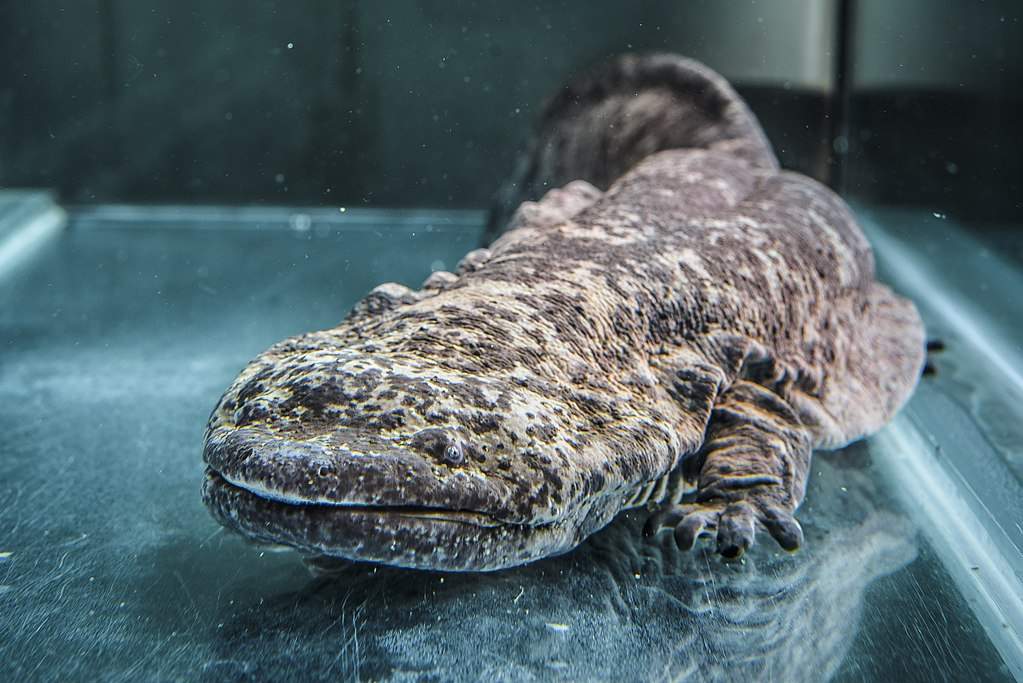
\includegraphics[width=0.8\textwidth]{img/home/chinese_giant_salamander.jpg}
    \caption*{Example of a figure. Image available \href{https://commons.wikimedia.org/wiki/File:Velemlok_\%C4\%8D\%C3\%ADnsk\%C3\%BD_zoo_praha_1.jpg}{here}.}
\end{figure}

\subsection*{Additional resources:}

\begin{itemize}
    \setlength\itemsep{-0.5em}
    \item \href{https://www.addgene.org/protocols/primer-design/}{AddGene: Primer design for PCR}
    \item \href{https://www.zymoresearch.com/blogs/blog/how-to-design-primers-for-pcr-experiments}{Zymo Research: How to Design Primers for PCR Experiments}
    \item \href{https://www.thermofisher.com/blog/behindthebench/pcr-primer-design-tips/}{ThermoFisher: PCR Primer Design Tips}
    \item \href{https://sharebiology.com/primer-designing-demonstration-step-by-step/}{Share Biology: Primer Designing – Demonstration step by step}
\end{itemize}

\end{document}